\section{Statistical analysis}
%
%%%%%%%%%%%%%%%%%%%%%%%%%%%%%%%%%%%%%%%%%%%%%%%%%%%%%%%%%%%
\subsection{Data} \label{s_sect:data}
%
%%%%%%%%%%%%%%%%%%%%%%%%%%%%%%%%%%%%
\subsubsection{Outcomes} \label{ss_sect:outcome}
%
On the one hand, the outcome from the \textbf{transcription task} was obtained following a two step procedure \citep{Boonen_et_al_2021}. First, we aligned the participant's orthographic  transcriptions at the utterance level. This step was repeated for every one of the \textcolor{blue}{$6400$ transcription ($64 \times 100$, see Section \ref{s_sect:JandT})}. Lastly, we computed the entropy measure of the aligned transcriptions using equation (\ref{eq:entropy}) \citep{Shannon_1948}. The last step resulted in $320$ entropy measures\footnote{\label{foot:doe}under DoE literature, the design corresponds to entropy measures for $32$ experimental units with $10$ replicate runs and $20$ duplicates, making a total of $320$ experimental runs.}.

Entropy was used as an objective measure of SI, i.e. a quantification of (dis)agreement between listeners' transcriptions. Utterances yielding a high degree of agreement between transcribers were considered highly intelligible and therefore registered a lower entropy $\left( H \rightarrow 0 \right)$, while utterances yielding a low degree of agreement were considered as exhibiting low intelligibility and therefore registered a higher entropy $\left( H \rightarrow 1 \right)$ \citep{Boonen_et_al_2021, Faes_et_al_2021}. In that sense, entropy was defined as: 
%
\begin{equation} \label{eq:entropy}
	H(\pmb{p}) = H = \frac{-\sum_{i=1}^{n} p_{i} \cdot \log_{2}(p_{i})}{\log_{2}(N)}
\end{equation}
%
where $N$ denotes the number of transcribers, $p_{i}$ the utterance's probability of occurrence, and $n$ the total number of events, i.e. two for the CJ-D case, and more than two for the CJ-O and HJ procedures.

On the other hand, the outcome for \textbf{judgment task} was obtained following the procedure outlined in Section \ref{ss_sect:proc}, with the total number of judgments per procedure detailed in Table \ref{tab:allocation}. 

\textcolor{blue}{It is important to mention that besides the exclusion of corrupted observations. e.g. no available rating, no other experimental run was eliminated before the modeling process. This decision departs from what it is observed in previous research}, e.g. \citet{Boonen_et_al_2020} decided to eliminate observations based on misfit analysis \citep{Lesterhuis_2018}, while \citet{vanDaal_2020} and \citet{Boonen_et_al_2021} did the same based on outlier analysis. For the case of misfit analysis, we argue that such procedures cannot be used without caution. The literature points out that in the context of CJ, these statistics are always relative, i.e. they depend on other stimulus and judges included in the assessment \citep{Pollitt_2012a, Pollitt_2012b}, while they have been proven to be less sensitive, as they are calculated with a low number of judgments per representation \citep{Pollitt_2012a}. On the other hand, for the case of outlier analysis, we argue that outlying observations cannot be identified properly outside the context of a full model \citep{McElreath_2020}, i.e. what can behave as an outlier based on a univariate analysis, can behave as expected under the appropriate model. Moreover, as stated by \citet{McElreath_2020}, outliers are interesting cases to analyze. \textcolor{blue}{Considering the previous, if we still manage to identify outlying observations within the context of the proposed models (see Section \ref{s_sect:models}), the researcher would rather adjust the model, so it can be robust against the influence of such outliers.}
%
%
%%%%%%%%%%%%%%%%%%%%%%%%%%%%%%%%%%%%
\subsubsection{Covariates} \label{ss_sect:covariates}
%
\textcolor{blue}{The sampled children registered the following characteristics regarding their hearing status:
	%
	\begin{enumerate}
		\item Normal Hearing (NHC)
		\item Hearing Impaired (HIC):
		\begin{itemize}
			\item Cochlear Implant (CIC) 
			\item Hearing Aid (HAC) 
			\item Auditory Brain stem Implant (ABI)
		\end{itemize}
	\end{enumerate}
}

\begin{comment}
	%%%%%%%%%%%%%%%%%%%%%%%%%%%%%%%%%%%%
	\textbf{for the experimenter:} Based on \citet{Faes_et_al_2021} we depict the procedure for the experimenter:
	%
	\begin{enumerate}
		\item 1. matching procedure 
		\item selection of suitable stimuli
		\item determine the number of stimuli per judge 
		\item 
	\end{enumerate}
	
	about matching procedure \citep{Faes_et_al_2021}:
	NH children were matched on gender, age and regional background, to the other two groups.Based on the previous NH kids were not representative of the NH population. 
	Question: How they were matched?, Propensity Score Matching or manual work?. 
	Age in NH at least has to be matched with "hearing age" in other groups, i.e. the length of use of the hearing device. However is still not completely appropriate. "lexical age", i.e. vocabulary size, is another matching measure (see p. 14 in \citep{Faes_et_al_2021} for more) 
	
\end{comment}
%
%
%%%%%%%%%%%%%%%%%%%%%%%%%%%%%%%%%%%%%%%%%%%%%%%%%%%%%%%%%%%
\subsection{Statistical modeling} \label{s_sect:models}
%
Considering the objectives outlined in Section \ref{seq:rq}, this section describes the model selection procedures and the statistical models considered.
%
%%%%%%%%%%%%%%%%%%%%%%%%%%%%%%%%%%%%
\subsubsection{Model selection}
%
Following the successful and comprehensive analysis in \citet{vanDaal_2020} and \citet{Lesterhuis_2018}, this research will also use the Information-Theoretic Approach (ITA) \citep{Anderson_2008, Chamberlain_1965} for the selection of competing models. 

First, we will translate our working hypotheses into statistical models. In the present research, this step will be supported by the use of Directed Acyclic Graphs (DAG) and probabilistic programming \citep{Jaynes_2003}. A DAG is the simplest representation of a Graphical Causal Models (GCM), a heuristic model that contains information not purely statistical, but unlike a detailed statistical model, it allow us to deduce which variable relationships can provide valid causal inferences \citep{Hernan_et_al_2020, McElreath_2020}, i.e. is a reasonable way to state our hypothesis, and make our assumption more transparent. However, abide by the "no-free lunch" rule, the causal inferences produced under a DAG are only valid if the assumed DAG is correct. On the other hand, the probabilistic programming will serve as the algebraic formalist to specify our probabilistic models.

Second, in order to select between competing models, we need to set an appropriate measure of what makes a model a better approximation of reality. \citet{McElreath_2020} goes all the way to argument that the best measure of model fit is the out-of-sample predictive accuracy. In that sense, this research will embrace the full flexibility of our bayesian implementation (see Section \ref{s_sect:estimation}) and use two criteria that provide a better approximations of the out-of-sample (cross-validated) deviance\footnote{\citet{vanDaal_2020} used the Akaike’s Information Criterion (AIC) \citep{Akaike_1974} with similar purposes.}: (1) the Widely Applicable Information Criterion (WAIC) \citep{Watanabe_2013}, and (2) the Pareto-smoothed importance sampling cross-validation (PSIC) \citep{Vehtari_et_al_2021}. 

Finally, considering the evidence in the previous step, we proceed to make inferences based on one or multiple models.
%
%
%%%%%%%%%%%%%%%%%%%%%%%%%%%%%%%%%%%%
\subsubsection{Models}
%
We will consider two interrelated models: (1) a measurement error model for entropy, and (2) a measurement model for the CJ and HJ procedures, respectively. \\

\noindent \textbf{Measurement error model for entropy:} \\
%
As it is described in Section \ref{ss_sect:outcome}, our data set is composed of $320$ entropy measures, nested within $32$ children with $10$ replicates per child. Each entropy measure was bounded in the continuum $[0,1]$, as expected from equation (\ref{eq:entropy}).

Previous research have already used the entropy measure as an outcome \citep{Boonen_et_al_2021, Faes_et_al_2021}. However, on those cases, the authors decided to aggregate the measure to a mean value, in order to ease its handling in modeling process. We argue this pre-aggregating procedure could be pernicious for a proper statistical inference, as "anytime we use an average value, discarding the uncertainty around that average, we risk overconfidence and spurious inference" \citep{McElreath_2020}. 

This claim is easier to understand using a though experiment within our research. For example, imagine we have two children with the same mean entropy, but the second child shows more variability in the measure than the first. It is clear from the example that the average entropy measure informs about the child's average SI, indicating that both children have a similar level. However, the variability around such mean entropy also informs about the child's SI, as a higher variability imply transcribers agreed less about the second child intelligibility across the $10$ utterances. A similiar intuition was presented in \citet{Boonen_et_al_2021}, but the paper only used the information in a descriptive analysis, rather than integrate it to the modeling process. 

We argue that the estimation of such measurement error model is trivial under the bayesian framework, and we present it in the following lines.

First, figure \ref{fig:entropy_ME} depicts the DAG representation of the model. The figure shows the $s$'th observed entropy measure $H^{O}_{is}$ nested within the $i$'th child, where $i=1, \dots, N_{c}$, $s=1, \dots, N_{s}$, with $N_{c} = 32$  and $N_{s} = 10$. Additionally, the figure reveals the observed entropy represents multiple instances of a "true" entropy $H^{T}_{i}$ for each child, but measured with error ($e_i$). Finally, we notice covariates are set to explain the "true" entropy.
%
\begin{figure}[h]
	\centering
	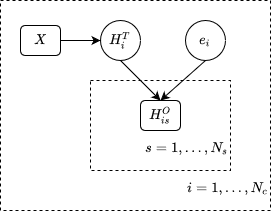
\includegraphics[width=0.4\linewidth]{entropy_ME.png}
	%
	\caption[DAG for the measurement error model of entropy.]%
	{DAG for the measurement error model of entropy. Circles represent latent variables, squares observed values or covariates, and large squares the nesting within specific units.}
	\label{fig:entropy_ME}
\end{figure}
%

\textcolor{red}{(in process)} \\

\begin{comment}
- Normal measurement error model: 
entropy_j ~ N( entropy_true_j, sigma_e) 

- In (Faes_et_al_2021) they use a random effects model for the entropy. 
entropy_j = entropy_true_j + error 
error ~ N( 0, sigma_e) 
* Notice both are the same (priors for entropy_true_j are needed) 

- Beta measurement error model: 
entropy_j ~ beta(alpha, beta) 
alpha = mu*M        ->  mu = alpha / M (mean) 
beta = (1 - mu)*M  ->  M = alpha + beta (prior sample size) 
* where mu = entropy_true_j and M is a distribution centered in 10 (utterances) 
\end{comment}
%
%
\noindent \textbf{Measurement models for the CJ and HJ procedures:} \\
%
\textcolor{red}{(in process)}

\begin{comment}
It will consider the correlation with the entropy measure.
%
\begin{enumerate}
	\item \textbf{Dichotomous CJ (CJ-D):} the Bradley-Terry-Luce model (BTL) \citep{Bradley_et_al_1952, Luce_1959}, used when the comparative judgments are dichotomous (CJ-D), 
	%
	\item \textbf{Ordinal CJ (CJ-O):} the Generalized Bradley-Terry-Luce model BTL(k) \citep{Tutz_1986, Agresti_1992}, used when the comparative ordinal CJ (CJ-O).
	%
	\item \textbf{Absolute (holistic) judgments (HJ):}
\end{enumerate}
\end{comment}
%
%
%%%%%%%%%%%%%%%%%%%%%%%%%%%%%%%%%%%%%%%%%%%%%%%%%%%%%%%%%%%
\subsection{Estimation procedure} \label{s_sect:estimation}
%
\textcolor{red}{(in process)}

\begin{comment}
We are going to work under the Bayesian framework, for details see latex code and variables to consider files. 

Identification of model:  
soft identification (see \citet{Depaoli_2021}) 

justification 
the benefits, and a comparison with the other options under the frequentist framework in \citet{Verhavert_2018}.
 
benefits:  
see master thesis, and \citet{Verhavert_2018} (p. 42-43) 


where \citep{Stan_2020} 
\end{comment}
%
%
%%%%%%%%%%%%%%%%%%%%%%%%%%%%%%%%%%%%%%%%%%%%%%%%%%%%%%%%%%%
\subsection{Evaluation}
%
%%%%%%%%%%%%%%%%%%%%%%%%%%%%%%%%%%%%
\subsubsection{validity}
%
\textcolor{red}{(in process)}

\begin{comment}
correlate latent scores (from different methods) with entropy measures (see research proposal)

\textbf{critique:} What about decision statements or think at loud rating process? (is it possible), \citet{Lesterhuis_2018} has shown their usefulness, while \citet{Boonen_et_al_2020} signals the need to know about the inner working of judgment processes.
\end{comment}
%
%
%%%%%%%%%%%%%%%%%%%%%%%%%%%%%%%%%%%%
\subsubsection{reliability}
%
\textcolor{red}{(in process)}

\begin{comment}
compare the Scale Separation Reliability (SSR, an inter-rater reliability measure), coming from CJ methods, with others for other methods

- No intra-rater reliability, also known as test-retest reliability (Verhavert_2018, Reliability_wiki_2022) 
- No Inter-method reliability,  assesses the degree to which test scores are consistent when there is a variation in the methods or instruments used (Verhavert_2018, Reliability_wiki_2022) 
- No comparison of SSR vs the true correlation of the latent scale and entropy measures 
* Justification: (Verhavert_2018, p. 156) " simulation studies could resolve the inconclusiveness regarding the SSR as a correlation with the truth."
\end{comment}
%
%
%%%%%%%%%%%%%%%%%%%%%%%%%%%%%%%%%%%%
\subsubsection{efficiency (time)}
%
\textcolor{red}{(in process)}

\begin{comment}
time needed for each judgement based on method from (Coertjens_et_al_2017).

statistical efficiency has been researched on \citet{Leijon_et_al_2019} and \citet{Pritikin_2020} for the bayesian dichotomous BTL model and the ordinal BTL model, respectively.
\end{comment}
%
%